\icode{E-MD-CA-L2-261111-005}
如图，光滑水平面上，质量为 \(M =\) \,\qty{2}{kg} 的木板 \(B\)（足够长），在 \(F =\) \,\qty{6}{N}的水平向右外力作用下从静止开始运动，\(t_0 =\) \,\qty{1}{s}末将一质量为 \(m =\) \,\qty{1}{kg}的煤块 \(A\) 轻放在 \(B\) 的右端，\(A\)、\(B\) 间动摩擦因数为 \(\mu = 0.3\)（最大静摩擦力等于滑动摩擦力，\(g =\) \,\qty{10}{m/s^2}），求：
\begin{enumerate}
	\item 煤块 \(A\) 刚放上时，\(A\)、\(B\) 的加速度大小；
	\item 煤块 \(A\) 在 \(B\) 上划过的痕迹的长度。
\end{enumerate}

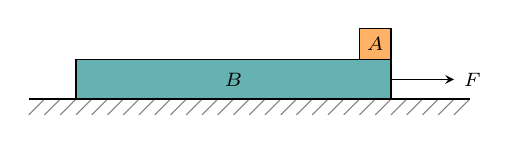
\begin{tikzpicture}[>=stealth,font=\scriptsize]
	\draw[fill=teal!60] (0,0) rectangle(4,.5)node[midway]{\(B\)};
	\draw[fill=orange!60] (3.6,.5) rectangle(4,.9)node[midway]{\(A\)};
	\draw[->] (4,.25)--++(.8,0)node[right]{\(F\)};
	\foreach \x in {-.6,-.4,...,5}
		\draw[gray] (\x,-.2)--++(.2,.2);
	\draw[thick] (-.6,0)--(5,0);
\end{tikzpicture}
\begin{answer}
	（1）\(a_A =\) \,\qty{3}{m/s^2} \(a_B =\) \,\qty{1.5}{m/s^2}（2）\qty{3}{m}
\end{answer}